\scanpage{23}
are isomorphic to subgroups of the group of exterior automorphisms of $\mathrm{G}$) ?

In a different direction, it would
% A thin pen trace rises from the top of the e, rather than from a supplied word space.
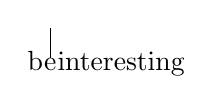
\begin{tikzpicture}[baseline=(e.base),x=1em,y=1ex]
  \node[anchor=base east,inner sep=0] (b) at (0,0) {b};
  \node[anchor=base west,inner sep=0] (e) at (0,0) {e};
  \node[anchor=base west,inner sep=0] at (e.base east) {interesting};
  \draw[line width=.25pt] (e.north) -- ++(0,2.5);
\end{tikzpicture}
to know more about the canonical morphism $\underline{\mathrm{g}}\handwritten{\longrightarrow}\underline{\mathrm{h}}/\mathrm{W}$, where $\underline{\mathrm{g}}$ is the Lie algebra of $\mathrm{G}$ and $\underline{\mathrm{h}}$ a Cartan subalgebra, and of the orbits of $\mathrm{G}$ on $\underline{\mathrm{g}}$, and the analoguous morphism of Steinberg $\mathrm{G}\handwritten{\longrightarrow}\mathrm{T}/\mathrm{W}$ and the orbits of $\mathrm{G}$ acting on itself. Do you know for instance exactly how varies the rank (= rang of the tangent map) of this \deleted{applic\unsure{at}i} map ? There are some reasons to believe that \deleted{this} for points of unipotent orbits of dimension
% The raised n- has typewriter-like serifs; its medium remains less certain than its letters.
% The curved pen leader and its separate low point are both retained.
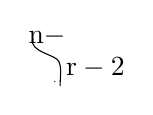
\begin{tikzpicture}[baseline=(r.base),x=1em,y=1ex]
  \node[anchor=base west,inner sep=0] (r) at (0,0) {$\mathrm{r}-2$};
  \node[anchor=base,inner sep=0] at (-.67,2.7) {$\inserted{\mathrm{n}-}$};
  \draw[line width=.4pt] (-1.18,3.15) .. controls (-1.35,2.0) and (-.32,1.8) .. (-.24,1.2) .. controls (-.13,.6) and (-.20,-.15) .. (-.20,-.85);
  \fill (-.39,-.47) circle (.25pt);
\end{tikzpicture}
(just

\begin{tikzpicture}[baseline=(live.base),x=1em,y=1ex]
  \node[anchor=base west,inner sep=0] at (0,1.45) {\deleted{the next lower after}};
  \node[anchor=base west,inner sep=0] (live) at (0,0) {\inserted{the next lower after}};
\end{tikzpicture}
the maximal dimension $\mathrm{n}-\mathrm{r}$), the rank is $\mathrm{r}-1$ in case all roots have same length (that is the corresponding diagrams
% These subscript cells preserve overlapping n/r contours without asserting their order.
$\mathrm{A}_{\unsure{\text{\begin{tikzpicture}[baseline=(an.base),x=1em,y=1ex]
  \node[anchor=base,inner sep=0] (an) at (0,0) {$\scriptstyle\mathrm{n}$};
  \node[anchor=base,inner sep=0] at (.09,.03) {$\scriptstyle\mathrm{r}$};
\end{tikzpicture}}}},
\mathrm{D}_{\unsure{\text{\begin{tikzpicture}[baseline=(dn.base),x=1em,y=1ex]
  \node[anchor=base,inner sep=0] (dn) at (0,0) {$\scriptstyle\mathrm{n}$};
  \node[anchor=base,inner sep=0] at (.07,-.04) {$\scriptstyle\mathrm{r}$};
  \draw[line width=.25pt] (.16,-.13) -- (.23,-.42);
\end{tikzpicture}}}},
\mathrm{E}_{\handwritten{6}},\mathrm{E}_{\handwritten{7}},\mathrm{E}_{\handwritten{8}}$
are those corresponding to Klein singularities), and $\handwritten{<}\mathrm{r}-1$ in
% The inserted all stands above the next line, with a curved leader ending before other.
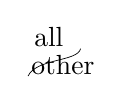
\begin{tikzpicture}[baseline=(other.base),x=1em,y=1ex]
  \node[anchor=base west,inner sep=0] (other) at (0,0) {other};
  \node[anchor=base,inner sep=0] at (.65,2.35) {\inserted{\handwritten{all}}};
  \draw[line width=.25pt] (1.8,2.2) .. controls (1.7,1.1) and (.2,1.4) .. (-.1,-.1);
\end{tikzpicture}
cases; in the first case, I would expect that there is just one orbit as stated, by the way, and maybe this property will be caracteristic of the ``homogene\deleted{a}ous'' case when all roots have same length. Also, what can be said of the dim%
% A low e and a raised rounded impression overlap; no correction chronology is assigned.
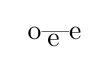
\begin{tikzpicture}[baseline=(de.base),x=1em,y=1ex]
  \node[anchor=base,inner sep=0] (de) at (0,0) {e};
  \node[anchor=base,inner sep=0] at (.035,.62) {\unsure{o|e}};
\end{tikzpicture}%
nsion of the set of all Borel subgroups containing a given element $\mathrm{g}\handwritten{\in}\mathrm{G}$, resp. whose Lie algebra contains a given element $\mathrm{x}\handwritten{\in}\underline{\mathrm{g}}$ ? If $2\mathrm{N}=\mathrm{n}-\mathrm{r}$ is the number of roots and if the dimension of the orbit of the given element is $2\mathrm{N}-2\mathrm{i}$, I would expect the dimension of the previous variety to be equal to $\mathrm{i}$; the inequality $\handwritten{\leqslant}\mathrm{i}$ would imply, by generalizing a depth argument of Br%
% Both crowded cells have i/e contours; their chronological order is not recoverable here.
\unsure{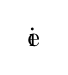
\begin{tikzpicture}[baseline=(bi.base),x=1em,y=1ex]
  \node[anchor=base,inner sep=0] (bi) at (0,0) {i};
  \node[anchor=base,inner sep=0] at (.04,-.02) {e};
\end{tikzpicture}}%
\unsure{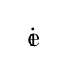
\begin{tikzpicture}[baseline=(be.base),x=1em,y=1ex]
  \node[anchor=base,inner sep=0] (be) at (0,0) {e};
  \node[anchor=base,inner sep=0] at (-.025,.02) {i};
\end{tikzpicture}}%
skorn, that the singularities of the fibers of your map $\underline{\mathrm{g}}\handwritten{\longrightarrow}\underline{\mathrm{h}}/\mathrm{W}$ (resp. Steinberg's $\mathrm{G}\handwritten{\longrightarrow}\mathrm{T}/\mathrm{W}$ in case $\mathrm{G}$ is simply connected instead of adjoint) are ``rational'', i.e. i%
% f and s share a cell; neither impression is silently discarded.
\unsure{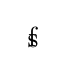
\begin{tikzpicture}[baseline=(iff.base),x=1em,y=1ex]
  \node[anchor=base,inner sep=0] (iff) at (0,0) {f};
  \node[anchor=base,inner sep=0] at (.025,-.02) {s};
\end{tikzpicture}}
$\mathrm{F}$ is such a fiber and $\mathrm{F}'\overset{\mathrm{f}}{\handwritten{\longrightarrow}}\mathrm{F}$ a resolution of singularities of $\mathrm{F}$, t%
% Two superposed h/e cells are retained without ordering the impressions.
\unsure{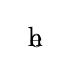
\begin{tikzpicture}[baseline=(th.base),x=1em,y=1ex]
  \node[anchor=base,inner sep=0] (th) at (0,0) {h};
  \node[anchor=base,inner sep=0] at (.02,-.02) {e};
\end{tikzpicture}}%
\unsure{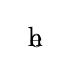
\begin{tikzpicture}[baseline=(te.base),x=1em,y=1ex]
  \node[anchor=base,inner sep=0] (te) at (0,0) {e};
  \node[anchor=base,inner sep=0] at (-.02,.02) {h};
\end{tikzpicture}}%
n $\mathrm{R}^{\mathrm{i}}\mathrm{f}_{\handwritten{*}}(\text{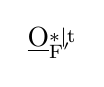
\begin{tikzpicture}[baseline=(oo.base),x=1em,y=1ex]
  \node[anchor=base,inner sep=0] (oo) at (0,0) {$\underline{\mathrm{O}}$};
  \node[anchor=base west,inner sep=0] at (.36,-1.02) {$\scriptstyle\mathrm{F}'$};
  \node[anchor=base west,inner sep=0] at (.36,.37) {$\scriptstyle\deleted{\unsure{*|\mathrm{t}}}$};
\end{tikzpicture}})=0$ for $\mathrm{i}\handwritten{>}0$. Maybe the ans\unsure{w|u}%
% A short upright trace above the e is retained; its relation to the letter is uncertain.
\unsure{\begin{tikzpicture}[baseline=(ae.base),x=1em,y=1ex]
  \node[anchor=base,inner sep=0] (ae) at (0,0) {e};
  \draw[line width=.3pt] ([xshift=-.12em]ae.north) -- ++(0,.62);
\end{tikzpicture}}%
r \deleted{\unsure{ot|to}}\handwritten{to} most of the questions I am asking are well known and I am just ignorant; for some of them, it would indeed be scandalous that the experts do not know the answer ! In any case, I would be grateful for any comment you would have on any of my questions.

Sincerely yours\\
\hspace*{.60\linewidth}\handwritten{A\,G\unsure{rothendieck}}\\
% A disconnected, interrupted vertical trace lies below the signature, towards the right.
% Its origin as ink versus a surface mark, and its function, remain uncertain.
\figure{\hspace*{6cm}\unsure{\begin{tikzpicture}[x=1mm,y=1mm]
  \fill (0,0) circle (.10pt);
  \draw[line width=.2pt] (0,-.5) -- (0,-1.5);
  \draw[line width=.2pt] (0,-2.0) -- (-.02,-3.4);
  \draw[line width=.2pt] (-.02,-4.2) -- (-.04,-5.3);
  \draw[line width=.2pt] (-.04,-5.8) -- (-.08,-7.0);
  \draw[line width=.12pt] (-.08,-7.4) -- (-.08,-8.0);
  \draw[line width=.2pt] (-.08,-8.2) -- (-.08,-8.8);
\end{tikzpicture}}}
% archive sheet number: 22
